\section{Experimental Results}
\label{sec:experiment}

To verify the feedback model, we conduct qualitative experiments on class neuron visualizations and quantitative evaluations on the weakly supervised object localization task. We use the three most popular pre-trained ConvNet models, AlexNet~\cite{Krizhevsky2012ImageNet}, VggNet~\cite{simonyan2013deep} and GoogleNet~\cite{Szegedy2014Going} for experiments. All three models are pre-trained with ImageNet 2012 classification training dataset~\cite{deng2009imagenet}, obtained from Caffe~\cite{jia2014caffe} model zoo. AlexNet achieves $\sim$15\% top 5 classification error on ImageNet 2012 testing dataset, while VggNet and GoogleNet obtains $\sim$7.5\%. GoogleNet slightly outperforms VggNet, but the gap is small and can be ignored. 

\subsection{Image Specific Class Model Visualization}
\label{subsec:visualization}
Given an image $I$, a class label $k$ and the hidden neuron activation states $\mathbf{z}$, we approximate the neural net class score $s_k$ with the first-order taylor expansion in the neighborhood of $I$:
\begin{equation}
  s_k(I, \mathbf{z}) \approx  \mathbf{T}_k(\mathbf{z})^T I + b
\end{equation}
where $\mathbf{T}_k(\mathbf{z})$ is the derivative of $s_k$ with respect to the image at the point of $I$ and $\mathbf{z}$. $\mathbf{T}_k(\mathbf{z})$ can be viewed as the linear template applied on image $I$ for measuring how likely the image belongs to class $k$. We can visualize $\mathbf{T}$ since it's the same size as the image $I$. We use this technique to visualize the our feedback model throughout the paper.

Specifically, for a VggNet which uses a stack of piecewise linear layers (\emph{i.e.} Conv, ReLU and max-pooling) to compute the class scores, once the hidden states $\mathbf{z}$ are determined, the final score is a linear function on the image, equivalent to the inner product between the template and the image.

\textbf{Comparison of Visualization Methods:} We compare the image gradient (template $\mathbf{T}$) after the feedback process against original gradient and Deconvolutional Neural Net (Deconv)~\cite{zeiler2014visualizing} on a set of complex images containing multiple objects from different classes. We show the qualititative results in Figure~\ref{fig:examples}. All techniques use the same pre-trained GoogleNet and ground truth class labels are given as a prior. The visualization results before feedback is the same as original image gradients, where all the hidden neurons states are determined by the bottom-up computations, while after feedback the visualizations are similar to Deconv. However, our feedback model captures more salient regions for the specific class while surpress irrelevant object area much better than Deconv.  

\textbf{Comparison of ConvNet Models:} We also qualitatively compare AlexNet, VggNet and Googlenet by visualizing their feedback templates in Figure~\ref{fig:model_compare}. All models are given the ground truth class labels as a prior. From the visualization results, we find that VggNet and GoogleNet produce more accurate visual attention than AlexNet, suggesting that using smaller convolution filters and deeper architectures could further distinguish similar and nearby objects. We also observe that, although both VggNet and GoogleNet produce very smilar image classification accuracies, GoogleNet better captures the salient object areas than VggNet. We hypothesize that the two 4096 dimensional fully connected layers (\emph{i.e.} fc6, fc7) in VggNet (which GoogleNet does not contain) could harm the spatial distinctiveness of the final image features,  

\textbf{Feedback Visualization of Similar Classes:} We also show a few intersting feedback visualizations for understanding the fine-grained classifcation models of GoogleNet. The GoogleNet is trained on ImageNet dataset with 1000 classes, among which there are $\sim$100 dog categories and $\sim$500 animal categories. We visualize the feedback templates of dog-cat images given paticular dog classes and animal classes in Figure~\ref{fig:class_compare}. We observe that each class has its own special salient image features for distinction, for example, some classes (\emph{i.e.} beagle, kit fox) look for local part features such as nose and ears, while others (\emph{i.e.} terrier, tiger) focus on global attributes such as furry and tabby.

\setlength{\tabcolsep}{0.5pt}
\begin{figure*}
\begin{center}
\begin{tabular}{ccccccc}
& \multicolumn{3}{c}{\small -------------------- Object 1: dog --------------------} & \multicolumn{3}{c}{\small -------------------- Object 2: cat --------------------} \\
\vspace{-2.5pt}
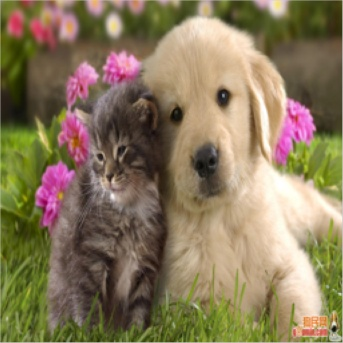
\includegraphics[width=0.14\linewidth,height=0.115\linewidth]{figs/examples/googlenet/oxford/dog-cat1} &
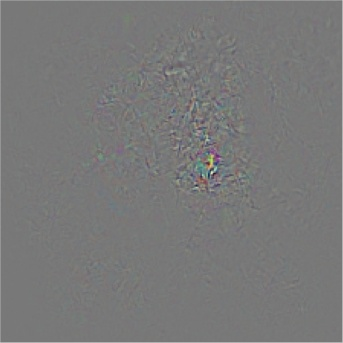
\includegraphics[width=0.14\linewidth,height=0.115\linewidth]{figs/examples/googlenet/oxford/dog-cat1_diff_258} &
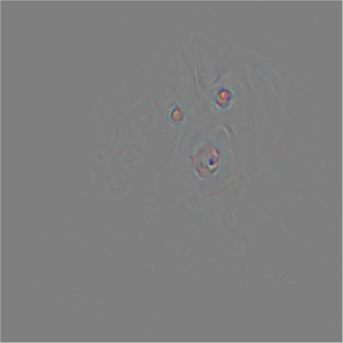
\includegraphics[width=0.14\linewidth,height=0.115\linewidth]{figs/examples/googlenet/deconv/dog-cat1_diff_258} &
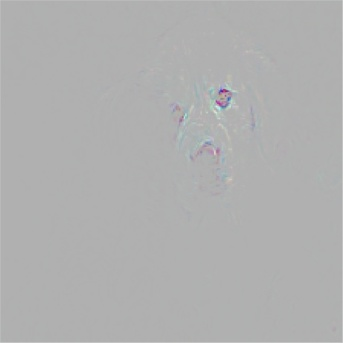
\includegraphics[width=0.14\linewidth,height=0.115\linewidth]{figs/examples/googlenet/soft/dog-cat1_diff_258} &
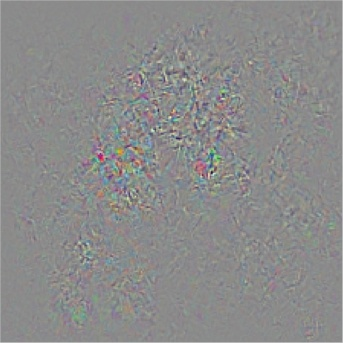
\includegraphics[width=0.14\linewidth,height=0.115\linewidth]{figs/examples/googlenet/oxford/dog-cat1_diff_286} &
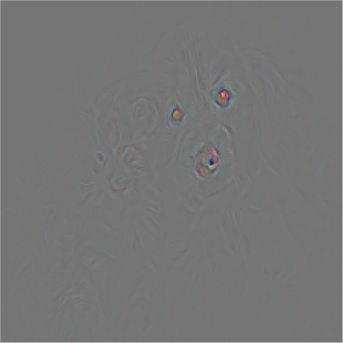
\includegraphics[width=0.14\linewidth,height=0.115\linewidth]{figs/examples/googlenet/deconv/dog-cat1_diff_286} &
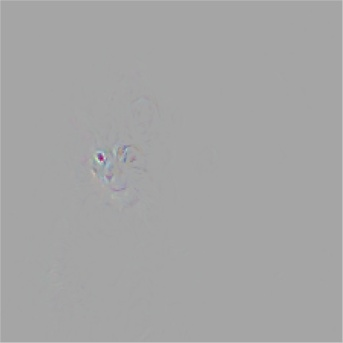
\includegraphics[width=0.14\linewidth,height=0.115\linewidth]{figs/examples/googlenet/soft/dog-cat1_diff_286} \\
\vspace{-2.5pt}
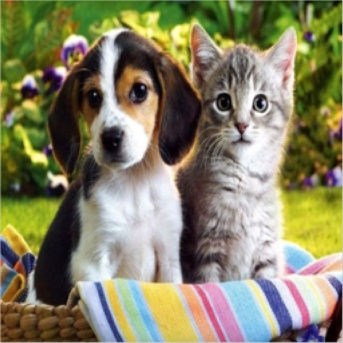
\includegraphics[width=0.14\linewidth,height=0.115\linewidth]{figs/examples/googlenet/oxford/dog-cat2} &
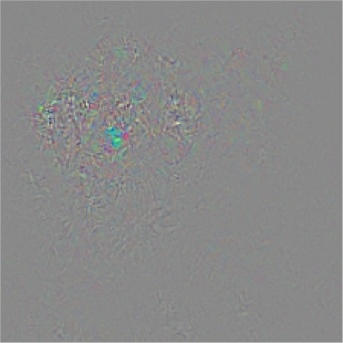
\includegraphics[width=0.14\linewidth,height=0.115\linewidth]{figs/examples/googlenet/oxford/dog-cat2_diff_163} &
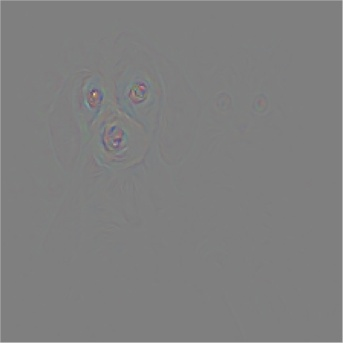
\includegraphics[width=0.14\linewidth,height=0.115\linewidth]{figs/examples/googlenet/deconv/dog-cat2_diff_163} &
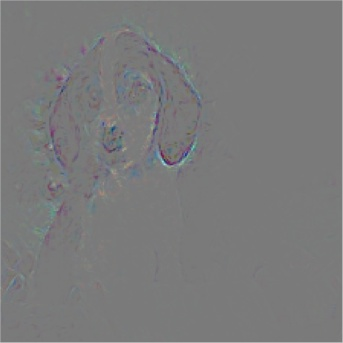
\includegraphics[width=0.14\linewidth,height=0.115\linewidth]{figs/examples/googlenet/soft/dog-cat2_diff_163} &
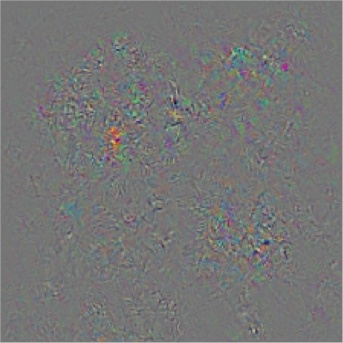
\includegraphics[width=0.14\linewidth,height=0.115\linewidth]{figs/examples/googlenet/oxford/dog-cat2_diff_286} &
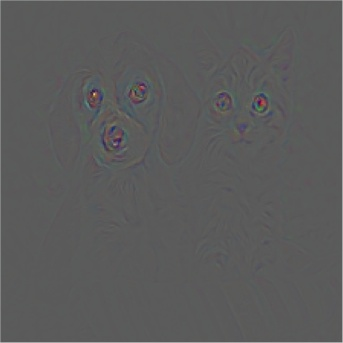
\includegraphics[width=0.14\linewidth,height=0.115\linewidth]{figs/examples/googlenet/deconv/dog-cat2_diff_286} &
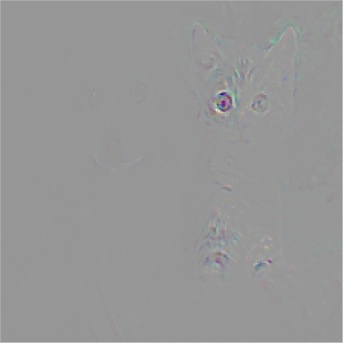
\includegraphics[width=0.14\linewidth,height=0.115\linewidth]{figs/examples/googlenet/soft/dog-cat2_diff_286} \\
\vspace{-2.5pt}
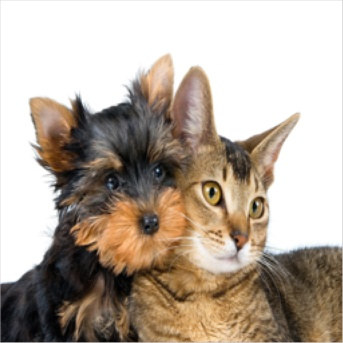
\includegraphics[width=0.14\linewidth,height=0.115\linewidth]{figs/examples/googlenet/oxford/dog-cat3} &
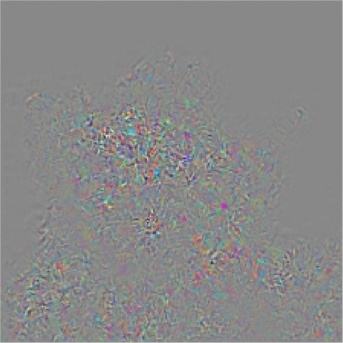
\includegraphics[width=0.14\linewidth,height=0.115\linewidth]{figs/examples/googlenet/oxford/dog-cat3_diff_188} &
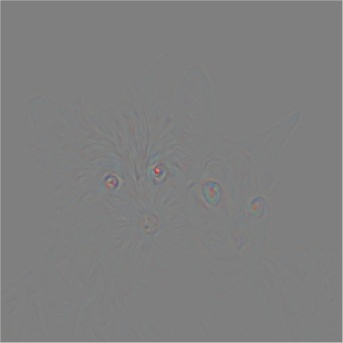
\includegraphics[width=0.14\linewidth,height=0.115\linewidth]{figs/examples/googlenet/deconv/dog-cat3_diff_188} &
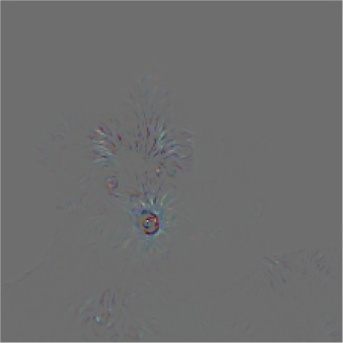
\includegraphics[width=0.14\linewidth,height=0.115\linewidth]{figs/examples/googlenet/soft/dog-cat3_diff_188} &
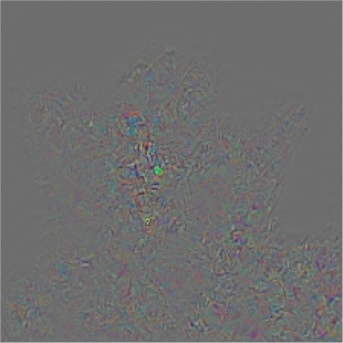
\includegraphics[width=0.14\linewidth,height=0.115\linewidth]{figs/examples/googlenet/oxford/dog-cat3_diff_286} &
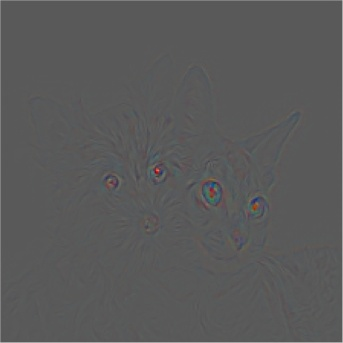
\includegraphics[width=0.14\linewidth,height=0.115\linewidth]{figs/examples/googlenet/deconv/dog-cat3_diff_286} &
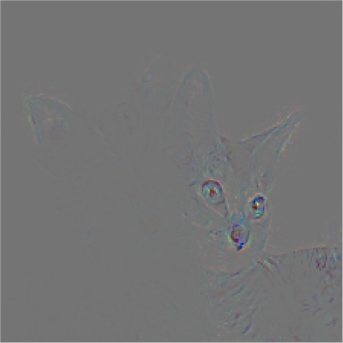
\includegraphics[width=0.14\linewidth,height=0.115\linewidth]{figs/examples/googlenet/soft/dog-cat3_diff_286} \\
\vspace{-2.5pt}
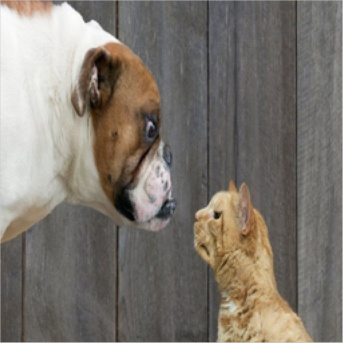
\includegraphics[width=0.14\linewidth,height=0.115\linewidth]{figs/examples/googlenet/oxford/dog-cat4} &
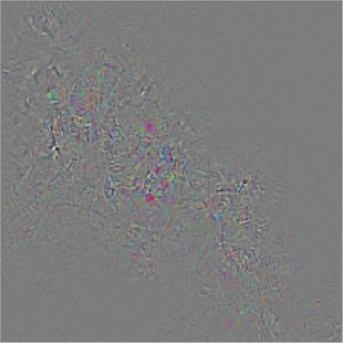
\includegraphics[width=0.14\linewidth,height=0.115\linewidth]{figs/examples/googlenet/oxford/dog-cat4_diff_243} &
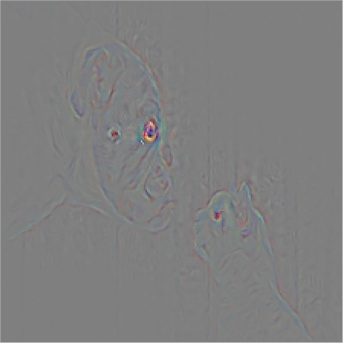
\includegraphics[width=0.14\linewidth,height=0.115\linewidth]{figs/examples/googlenet/deconv/dog-cat4_diff_243} &
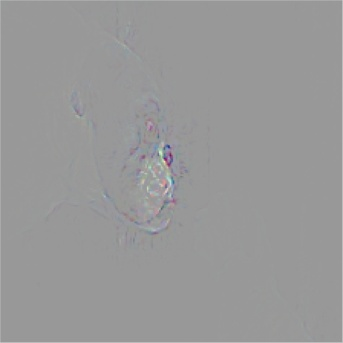
\includegraphics[width=0.14\linewidth,height=0.115\linewidth]{figs/examples/googlenet/soft/dog-cat4_diff_243} &
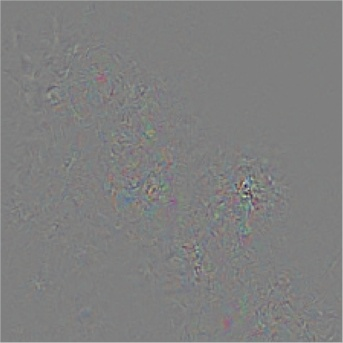
\includegraphics[width=0.14\linewidth,height=0.115\linewidth]{figs/examples/googlenet/oxford/dog-cat4_diff_286} &
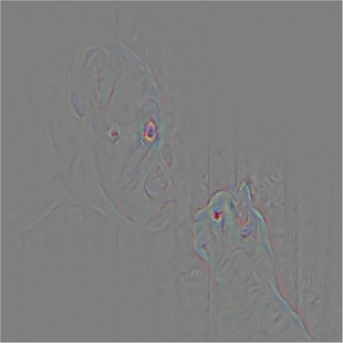
\includegraphics[width=0.14\linewidth,height=0.115\linewidth]{figs/examples/googlenet/deconv/dog-cat4_diff_286} &
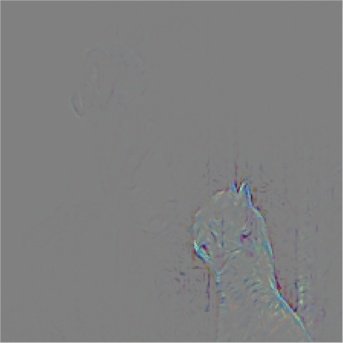
\includegraphics[width=0.14\linewidth,height=0.115\linewidth]{figs/examples/googlenet/soft/dog-cat4_diff_286} \\
& \multicolumn{3}{c}{\small -------------------- Object 1: car --------------------} & \multicolumn{3}{c}{\small -------------------- Object 2: bike --------------------} \\
\vspace{-2.5pt}
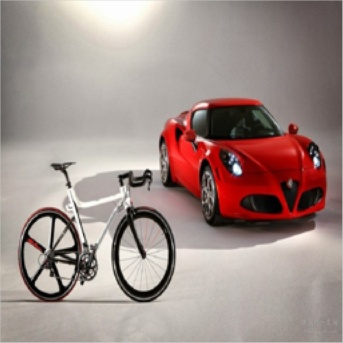
\includegraphics[width=0.14\linewidth,height=0.115\linewidth]{figs/examples/googlenet/oxford/bic-car1} &
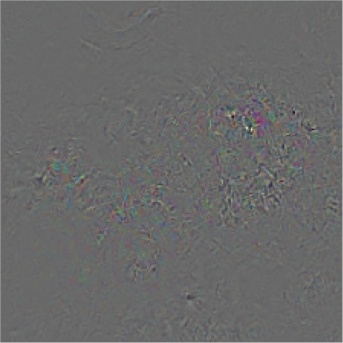
\includegraphics[width=0.14\linewidth,height=0.115\linewidth]{figs/examples/googlenet/oxford/bic-car1_diff_818} &
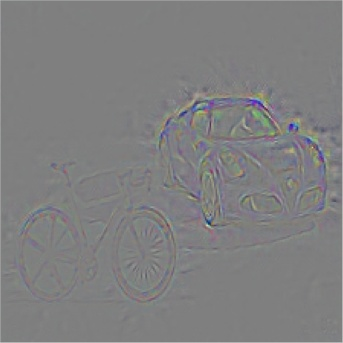
\includegraphics[width=0.14\linewidth,height=0.115\linewidth]{figs/examples/googlenet/deconv/bic-car1_diff_818} &
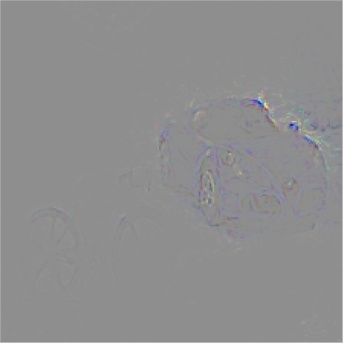
\includegraphics[width=0.14\linewidth,height=0.115\linewidth]{figs/examples/googlenet/soft/bic-car1_diff_818} &
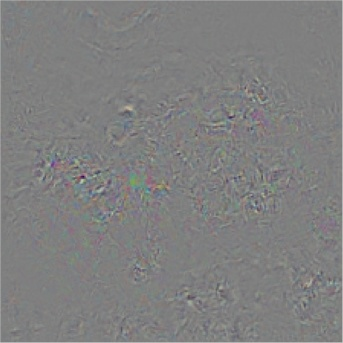
\includegraphics[width=0.14\linewidth,height=0.115\linewidth]{figs/examples/googlenet/oxford/bic-car1_diff_672} &
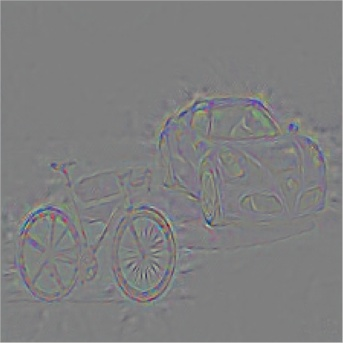
\includegraphics[width=0.14\linewidth,height=0.115\linewidth]{figs/examples/googlenet/deconv/bic-car1_diff_672} &
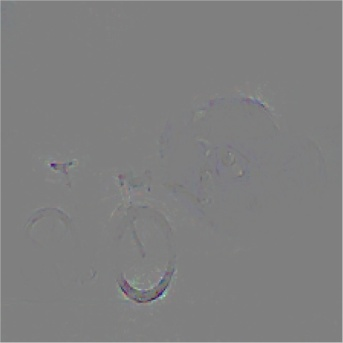
\includegraphics[width=0.14\linewidth,height=0.115\linewidth]{figs/examples/googlenet/soft/bic-car1_diff_672} \\
\vspace{-2.5pt}
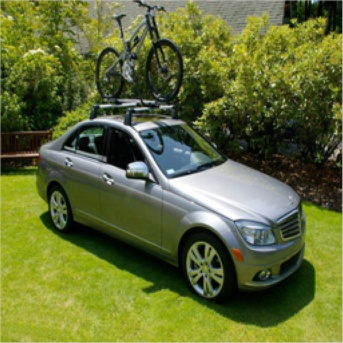
\includegraphics[width=0.14\linewidth,height=0.115\linewidth]{figs/examples/googlenet/oxford/bic-car2} &
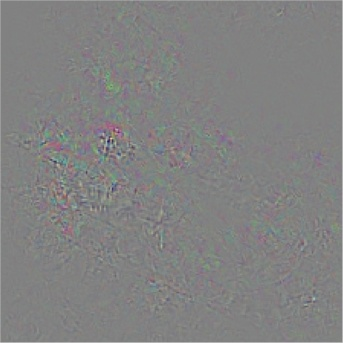
\includegraphics[width=0.14\linewidth,height=0.115\linewidth]{figs/examples/googlenet/oxford/bic-car2_diff_818} &
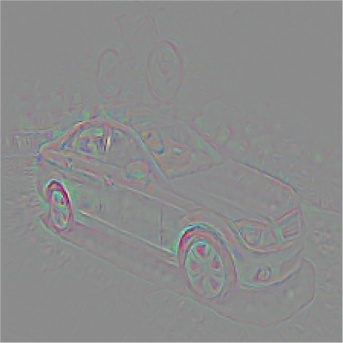
\includegraphics[width=0.14\linewidth,height=0.115\linewidth]{figs/examples/googlenet/deconv/bic-car2_diff_818} &
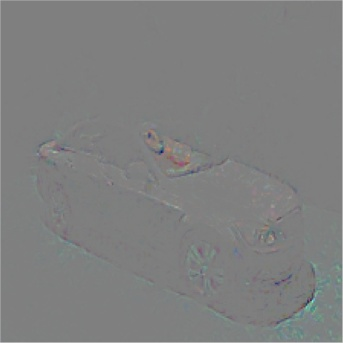
\includegraphics[width=0.14\linewidth,height=0.115\linewidth]{figs/examples/googlenet/soft/bic-car2_diff_818} &
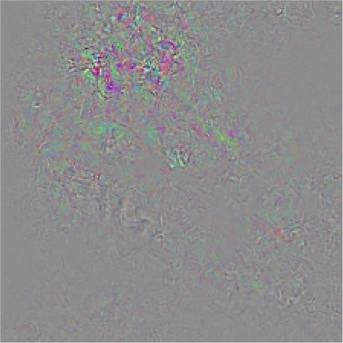
\includegraphics[width=0.14\linewidth,height=0.115\linewidth]{figs/examples/googlenet/oxford/bic-car2_diff_672} &
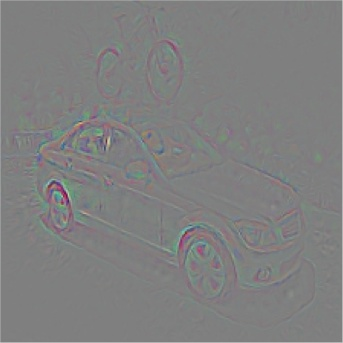
\includegraphics[width=0.14\linewidth,height=0.115\linewidth]{figs/examples/googlenet/deconv/bic-car2_diff_672} &
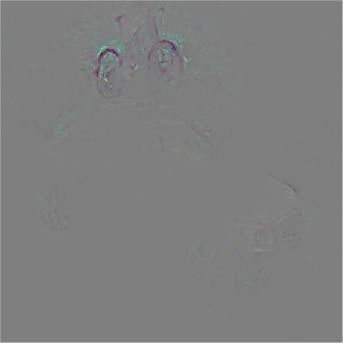
\includegraphics[width=0.14\linewidth,height=0.115\linewidth]{figs/examples/googlenet/soft/bic-car2_diff_672} \\
& \multicolumn{3}{c}{\small -------------------- Object 1: zebra --------------------} & \multicolumn{3}{c}{\small -------------------- Object 2: elephant --------------------} \\
\vspace{-2.5pt}
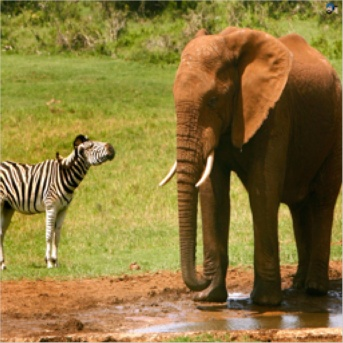
\includegraphics[width=0.14\linewidth,height=0.115\linewidth]{figs/examples/googlenet/oxford/zeb-ele1} &
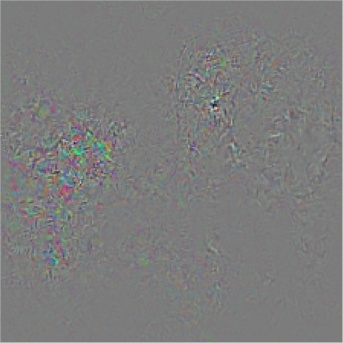
\includegraphics[width=0.14\linewidth,height=0.115\linewidth]{figs/examples/googlenet/oxford/zeb-ele1_diff_341} &
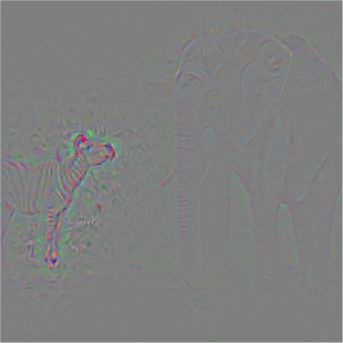
\includegraphics[width=0.14\linewidth,height=0.115\linewidth]{figs/examples/googlenet/deconv/zeb-ele1_diff_341} &
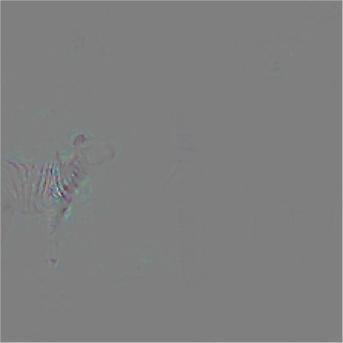
\includegraphics[width=0.14\linewidth,height=0.115\linewidth]{figs/examples/googlenet/soft/zeb-ele1_diff_341} &
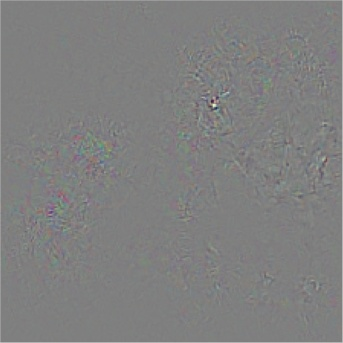
\includegraphics[width=0.14\linewidth,height=0.115\linewidth]{figs/examples/googlenet/oxford/zeb-ele1_diff_387} &
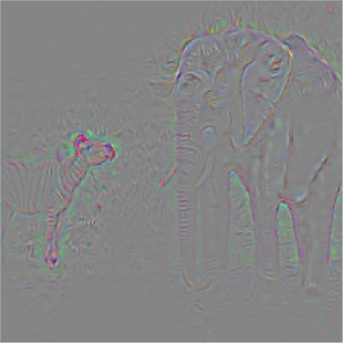
\includegraphics[width=0.14\linewidth,height=0.115\linewidth]{figs/examples/googlenet/deconv/zeb-ele1_diff_387} &
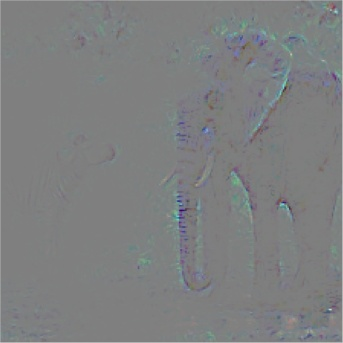
\includegraphics[width=0.14\linewidth,height=0.115\linewidth]{figs/examples/googlenet/soft/zeb-ele1_diff_387} \\
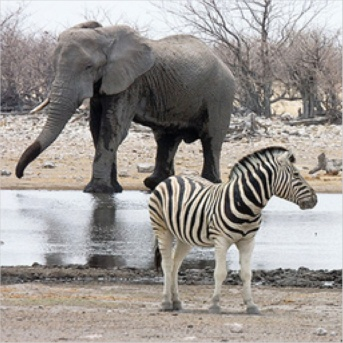
\includegraphics[width=0.14\linewidth,height=0.115\linewidth]{figs/examples/googlenet/oxford/zeb-ele2} &
\includegraphics[width=0.14\linewidth,height=0.115\linewidth]{figs/examples/googlenet/oxford/zeb-ele2_diff_341} &
\includegraphics[width=0.14\linewidth,height=0.115\linewidth]{figs/examples/googlenet/deconv/zeb-ele2_diff_341} &
\includegraphics[width=0.14\linewidth,height=0.115\linewidth]{figs/examples/googlenet/soft/zeb-ele2_diff_341} &
\includegraphics[width=0.14\linewidth,height=0.115\linewidth]{figs/examples/googlenet/oxford/zeb-ele2_diff_387} &
\includegraphics[width=0.14\linewidth,height=0.115\linewidth]{figs/examples/googlenet/deconv/zeb-ele2_diff_387} &
\includegraphics[width=0.14\linewidth,height=0.115\linewidth]{figs/examples/googlenet/soft/zeb-ele2_diff_387} \\
{\small (a) Image} &
{\small (b) Gradient} &
{\small (c) Deconv} &
{\small (d) Feedback} &
{\small (e) Gradient} &
{\small (f) Deconv} &
{\small (g) Feedback} \\
\end{tabular}
% \vspace{-10pt}
\caption{We demonstrate the effectiveness of feedback neural networks for class-specific feature extraction, by comparing the class model visualization results against original gradient~\cite{simonyan2013deep} and Deconv~\cite{zeiler2014visualizing} on selected images with multiple objects. All methods compute visualizations using a pre-trained GoogleNet trained on ImageNet 2012 classification dataset. Column (a) shows the input images (\emph{i.e.} dog v.s. cat, car v.s. bike, and zebra v.s. elephant). Column (b) and (e) show the original image gradients given the provided class labels. Column (c) and (f) show the Deconv results. Column (d) and (g) show the image gradients after feedback. Comparing against original gradient and Deconv, the feedback visualization captures more accurate salient area of the target object. For example, in the 4th row, both original template and Deconv see the dog and cat, even provided with the target label. In the last row, when zebra is specified, Deconv finds it hard to supress the elephant area. Our feedback method supress the irrelevant object much better. Better viewed in color and zoom in.} 
\label{fig:examples}
% \vspace{-30pt}
\end{center}
\end{figure*}

\setlength{\tabcolsep}{0.5pt}
\begin{figure*}
\begin{center}
\begin{tabular}{ccccccc}
%\rotatebox{90}{\hspace{5mm}Gradient} &
\vspace{-2.5pt}
\includegraphics[width=0.14\linewidth,height=0.115\linewidth]{figs/examples/googlenet/soft/zeb-ele1} &
\includegraphics[width=0.14\linewidth,height=0.115\linewidth]{figs/examples/alexnet/soft/zeb-ele1_diff_341} &
\includegraphics[width=0.14\linewidth,height=0.115\linewidth]{figs/examples/vggnet/soft/zeb-ele1_diff_341} &
\includegraphics[width=0.14\linewidth,height=0.115\linewidth]{figs/examples/googlenet/soft/zeb-ele1_diff_341} &
\includegraphics[width=0.14\linewidth,height=0.115\linewidth]{figs/examples/alexnet/soft/zeb-ele1_diff_387} &
\includegraphics[width=0.14\linewidth,height=0.115\linewidth]{figs/examples/vggnet/soft/zeb-ele1_diff_387} &
\includegraphics[width=0.14\linewidth,height=0.115\linewidth]{figs/examples/googlenet/soft/zeb-ele1_diff_387} \\
%\rotatebox{90}{\hspace{5mm}Saliency} &
\vspace{-2.5pt}
\includegraphics[width=0.14\linewidth,height=0.115\linewidth]{figs/examples/googlenet/soft/zeb-ele1} &
\includegraphics[width=0.14\linewidth,height=0.115\linewidth]{figs/examples/alexnet/soft/zeb-ele1_sali_341} &
\includegraphics[width=0.14\linewidth,height=0.115\linewidth]{figs/examples/vggnet/soft/zeb-ele1_sali_341} &
\includegraphics[width=0.14\linewidth,height=0.115\linewidth]{figs/examples/googlenet/soft/zeb-ele1_sali_341} &
\includegraphics[width=0.14\linewidth,height=0.115\linewidth]{figs/examples/alexnet/soft/zeb-ele1_sali_387} &
\includegraphics[width=0.14\linewidth,height=0.115\linewidth]{figs/examples/vggnet/soft/zeb-ele1_sali_387} &
\includegraphics[width=0.14\linewidth,height=0.115\linewidth]{figs/examples/googlenet/soft/zeb-ele1_sali_387} \\
%\rotatebox{90}{\hspace{5mm}Gradient} &
\vspace{-2.5pt}
\includegraphics[width=0.14\linewidth,height=0.115\linewidth]{figs/examples/googlenet/soft/zeb-ele2} &
\includegraphics[width=0.14\linewidth,height=0.115\linewidth]{figs/examples/alexnet/soft/zeb-ele2_diff_341} &
\includegraphics[width=0.14\linewidth,height=0.115\linewidth]{figs/examples/vggnet/soft/zeb-ele2_diff_341} &
\includegraphics[width=0.14\linewidth,height=0.115\linewidth]{figs/examples/googlenet/soft/zeb-ele2_diff_341} &
\includegraphics[width=0.14\linewidth,height=0.115\linewidth]{figs/examples/alexnet/soft/zeb-ele2_diff_387} &
\includegraphics[width=0.14\linewidth,height=0.115\linewidth]{figs/examples/vggnet/soft/zeb-ele2_diff_387} &
\includegraphics[width=0.14\linewidth,height=0.115\linewidth]{figs/examples/googlenet/soft/zeb-ele2_diff_387} \\
%\rotatebox{90}{\hspace{5mm}Saliency} &
\includegraphics[width=0.14\linewidth,height=0.115\linewidth]{figs/examples/googlenet/soft/zeb-ele2} &
\includegraphics[width=0.14\linewidth,height=0.115\linewidth]{figs/examples/alexnet/soft/zeb-ele2_sali_341} &
\includegraphics[width=0.14\linewidth,height=0.115\linewidth]{figs/examples/vggnet/soft/zeb-ele2_sali_341} &
\includegraphics[width=0.14\linewidth,height=0.115\linewidth]{figs/examples/googlenet/soft/zeb-ele2_sali_341} &
\includegraphics[width=0.14\linewidth,height=0.115\linewidth]{figs/examples/alexnet/soft/zeb-ele2_sali_387} &
\includegraphics[width=0.14\linewidth,height=0.115\linewidth]{figs/examples/vggnet/soft/zeb-ele2_sali_387} &
\includegraphics[width=0.14\linewidth,height=0.115\linewidth]{figs/examples/googlenet/soft/zeb-ele2_sali_387} \\
%\rotatebox{90}{\hspace{5mm}Gradient} &
%\includegraphics[width=0.13\linewidth]{figs/examples/googlenet/soft/bic-car1} &
%\includegraphics[width=0.13\linewidth]{figs/examples/alexnet/soft/bic-car1_diff_818} &
%\includegraphics[width=0.13\linewidth]{figs/examples/vggnet/soft/bic-car1_diff_818} &
%\includegraphics[width=0.13\linewidth]{figs/examples/googlenet/soft/bic-car1_diff_818} &
%\includegraphics[width=0.13\linewidth]{figs/examples/alexnet/soft/bic-car1_diff_672} &
%\includegraphics[width=0.13\linewidth]{figs/examples/vggnet/soft/bic-car1_diff_672} &
%\includegraphics[width=0.13\linewidth]{figs/examples/googlenet/soft/bic-car1_diff_672} \\
%\rotatebox{90}{\hspace{5mm}Saliency} &
%\includegraphics[width=0.13\linewidth]{figs/examples/googlenet/soft/bic-car1} &
%\includegraphics[width=0.13\linewidth]{figs/examples/alexnet/soft/bic-car1_sali_818} &
%\includegraphics[width=0.13\linewidth]{figs/examples/vggnet/soft/bic-car1_sali_818} &
%\includegraphics[width=0.13\linewidth]{figs/examples/googlenet/soft/bic-car1_sali_818} &
%\includegraphics[width=0.13\linewidth]{figs/examples/alexnet/soft/bic-car1_sali_672} &
%\includegraphics[width=0.13\linewidth]{figs/examples/vggnet/soft/bic-car1_sali_672} &
%\includegraphics[width=0.13\linewidth]{figs/examples/googlenet/soft/bic-car1_sali_672} \\
%\rotatebox{90}{\hspace{5mm}Gradient} &
%\includegraphics[width=0.13\linewidth]{figs/examples/googlenet/soft/bic-car2} &
%\includegraphics[width=0.13\linewidth]{figs/examples/alexnet/soft/bic-car2_diff_818} &
%\includegraphics[width=0.13\linewidth]{figs/examples/vggnet/soft/bic-car2_diff_818} &
%\includegraphics[width=0.13\linewidth]{figs/examples/googlenet/soft/bic-car2_diff_818} &
%\includegraphics[width=0.13\linewidth]{figs/examples/alexnet/soft/bic-car2_diff_672} &
%\includegraphics[width=0.13\linewidth]{figs/examples/vggnet/soft/bic-car2_diff_672} &
%\includegraphics[width=0.13\linewidth]{figs/examples/googlenet/soft/bic-car2_diff_672} \\
%\rotatebox{90}{\hspace{5mm}Saliency} &
%\includegraphics[width=0.13\linewidth]{figs/examples/googlenet/soft/bic-car2} &
%\includegraphics[width=0.13\linewidth]{figs/examples/alexnet/soft/bic-car2_sali_818} &
%\includegraphics[width=0.13\linewidth]{figs/examples/vggnet/soft/bic-car2_sali_818} &
%\includegraphics[width=0.13\linewidth]{figs/examples/googlenet/soft/bic-car2_sali_818} &
%\includegraphics[width=0.13\linewidth]{figs/examples/alexnet/soft/bic-car2_sali_672} &
%\includegraphics[width=0.13\linewidth]{figs/examples/vggnet/soft/bic-car2_sali_672} &
%\includegraphics[width=0.13\linewidth]{figs/examples/googlenet/soft/bic-car2_sali_672} \\
{\small (a) Image} &
{\small (b) AlexNet} &
{\small (c) VggNet} &
{\small (d) GoogleNet} &
{\small (e) AlexNet} &
{\small (f) VggNet} &
{\small (g) GoogleNet} \\
\end{tabular}
% \vspace{-10pt}
\caption{We visualize the feedback ability of three most popular pre-trained ConvNets: AlexNet, VggNet and GoogleNet, by visualizing the final image gradients and salience maps after feedback. We show the input images in column (a). We show the results of the three models feedbacked by "zebra" in column (b), (c), (d) and by "elephant" in column (e), (f), (g) repsectively. We find that VggNet performs quite better than AlexNet, especially in capturing salient object details, suggesting the benefit of usage of small convolutional filters and deeper architecture. Although both VggNet and GogoleNet produce similar classification accruacy, we find GoogleNet provides the better class specific feature separations. We suspect the two 4096 fully connected layers in VggNet (which GoogleNetdoes not have) could harm the spatial distinctiveness of image features.}
\label{fig:model_compare}
% \vspace{-30pt}
\end{center}
\end{figure*}

\setlength{\tabcolsep}{0.5pt}
\begin{figure*}
\begin{center}
\begin{tabular}{ccccccc}
{\small (a) Image} &
{\small (b) G. pyrenees} &
{\small (c) Beagle} &
{\small (d) York. terrier} &
{\small (e) Kit fox} &
{\small (f) Tiger} &
{\small (g) Ostrich} \\
\vspace{-2.5pt}
&
\includegraphics[width=0.14\linewidth,height=0.08\linewidth]{figs/class_compare/pyrenees} &
\includegraphics[width=0.14\linewidth,height=0.08\linewidth]{figs/class_compare/beagle} &
\includegraphics[width=0.14\linewidth,height=0.08\linewidth]{figs/class_compare/yorkshire-terrier} &
\includegraphics[width=0.14\linewidth,height=0.08\linewidth]{figs/class_compare/kit-fox} &
\includegraphics[width=0.14\linewidth,height=0.08\linewidth]{figs/class_compare/tiger} &
\includegraphics[width=0.14\linewidth,height=0.08\linewidth]{figs/class_compare/ostrich} \\
\vspace{-2.5pt}
\includegraphics[width=0.14\linewidth,height=0.115\linewidth]{figs/class_compare/googlenet/soft/dog-cat1} &
\includegraphics[width=0.14\linewidth,height=0.115\linewidth]{figs/class_compare/googlenet/soft/dog-cat1_diff_258} &
\includegraphics[width=0.14\linewidth,height=0.115\linewidth]{figs/class_compare/googlenet/soft/dog-cat1_diff_163} &
\includegraphics[width=0.14\linewidth,height=0.115\linewidth]{figs/class_compare/googlenet/soft/dog-cat1_diff_188} &
\includegraphics[width=0.14\linewidth,height=0.115\linewidth]{figs/class_compare/googlenet/soft/dog-cat1_diff_279} &
\includegraphics[width=0.14\linewidth,height=0.115\linewidth]{figs/class_compare/googlenet/soft/dog-cat1_diff_293} &
\includegraphics[width=0.14\linewidth,height=0.115\linewidth]{figs/class_compare/googlenet/soft/dog-cat1_diff_10} \\
\vspace{-2.5pt}
\includegraphics[width=0.14\linewidth,height=0.115\linewidth]{figs/class_compare/googlenet/soft/dog-cat2} &
\includegraphics[width=0.14\linewidth,height=0.115\linewidth]{figs/class_compare/googlenet/soft/dog-cat2_diff_258} &
\includegraphics[width=0.14\linewidth,height=0.115\linewidth]{figs/class_compare/googlenet/soft/dog-cat2_diff_163} &
\includegraphics[width=0.14\linewidth,height=0.115\linewidth]{figs/class_compare/googlenet/soft/dog-cat2_diff_188} &
\includegraphics[width=0.14\linewidth,height=0.115\linewidth]{figs/class_compare/googlenet/soft/dog-cat2_diff_279} &
\includegraphics[width=0.14\linewidth,height=0.115\linewidth]{figs/class_compare/googlenet/soft/dog-cat2_diff_293} &
\includegraphics[width=0.14\linewidth,height=0.115\linewidth]{figs/class_compare/googlenet/soft/dog-cat2_diff_10} \\
\includegraphics[width=0.14\linewidth,height=0.115\linewidth]{figs/class_compare/googlenet/soft/dog-cat3} &
\includegraphics[width=0.14\linewidth,height=0.115\linewidth]{figs/class_compare/googlenet/soft/dog-cat3_diff_258} &
\includegraphics[width=0.14\linewidth,height=0.115\linewidth]{figs/class_compare/googlenet/soft/dog-cat3_diff_163} &
\includegraphics[width=0.14\linewidth,height=0.115\linewidth]{figs/class_compare/googlenet/soft/dog-cat3_diff_188} &
\includegraphics[width=0.14\linewidth,height=0.115\linewidth]{figs/class_compare/googlenet/soft/dog-cat3_diff_279} &
\includegraphics[width=0.14\linewidth,height=0.115\linewidth]{figs/class_compare/googlenet/soft/dog-cat3_diff_293} &
\includegraphics[width=0.14\linewidth,height=0.115\linewidth]{figs/class_compare/googlenet/soft/dog-cat3_diff_10} \\
\end{tabular}
% \vspace{-10pt}
\caption{We show some interesting visualizations for the understanding of fine-grained classification by comparsing against the feedback gradients of ground truth labels and other classes. The top row shows the class labels and a representative image for each class for the ease of understanding. Column (a) shows the three examplar input images, their ground truth labels are great pyrenees, beagle and yorkshire terrier respectively. We can see that although (b), (c) and (d) are all dogs, their salient area for distinction are quite different. Noses are one of the most important feature for classifying dogs, but ears are specific feature for beagles, while fluffy is more importatnt to yorkshire terrier. When the top down is from (e) kit fox, features on the cat in the last row is more fox-specific: nose and ears. When top down is from (f) tiger, features on the same at is more tiger-specific: textures. And when it's (g) ostrich, nothing special come out.}
\label{fig:class_compare}
% \vspace{-30pt}
\end{center}
\end{figure*}

\subsection{Weakly Supervised Object Localization}
\label{subsec:localization}
To quantitatively demonstrate the effectiveness of the feedback model. we experiment on the ImageNet 2014 localization task.

As pointed in~\cite{simonyan2013deep}, the magnitude of the elements in the model template $\mathbf{T}_k$ defines the class specific salience map on image $I$. Pixels with larger magnitudes indicate that they are more important to the class. We adopt the same saliency extraction strategy as~\cite{simonyan2013deep} that a single class saliency value $M_k$ for class $k$ at pixel $(i,j)$ is computed across all color channels: $M_k(i,j) = \max_{c \in rgb} | T_k(i,j,c) |$.

Although the three ConvNets are pre-trained for image classification, we could use the feedbacked salience map for weakly supervised object localization. Following~\cite{simonyan2013deep}, given an image and the corresponding class salience map, we compute the object segmentation mask using the GraphCut color segmentation~\cite{yuri2001interactive}. During the inialization of graph cut, We set the pixels with the saliency higher than 95\% quantile of the saliency distribution in the image as foreground and those with the saliency lower than 30\% quantile as background. Once foreground and background segmentations are computed, the object segmentation mask is set to the largest connected component of the foreground pixels and the tighest bounding box is extracted as the localization result.

We test our localization results on ImageNet 2014 localization validation set, which contains $\sim$20000 images with each image associated with a label and a bounding box. The predicted bounding box is considered as correct if its overlap with the ground truth is over 50\%. We resize every image to 224x224 as the models' required resolution and provide the ground-truth class labels for the localization prediction. No further preprocessing or multi-scale strategy is involved. 

\textbf{Comparison of Localization Methods:} Table~\ref{tab:localization_accuracy} shows the comparsion of weakly supervised localization accuracy against Oxford and Deconv. We use the same VggNet and apply the same graph cut strategy on all the 3 models. Our method obtains 57\% accuracy, outperforming both Oxford 50\% and Deconv 53\%, suggesting that in terms of capturing attention and localizing salient objects, our feedback net is better. Note that currently this is only top-down and weakly supervised and the object localization task is not taken into account during training.

\textbf{Comparsion of ConvNet Models:} We also compare the weakly supervised localization ability of the three most popular ConvNet models: AlexNet, VggNet and GoogleNet in Table~\ref{tab:localization_model_compare}, given the ground-truth class labels. AlexNet ... \textbf{\color{red} I need the number to complete the paragraph. } 

However, Most of the images in ImageNet 2014 dataset contain only one salient object. We further show some localization results on images with multiple object classes in Figure~\ref{} ... \textbf{\color{red} I need the figures to complete the paragraph}. Obviously our feedback net cannot distinguish multiple object instances from the same class, but could capture the salient areas, which could be utilized by other sophisticated object detection algorithms. 

\begin{table}
\centering
\small
Localization Errors of Given Ground Truth Labels
\begin{tabular}{|c|c|}
\hline
Method & Localization Error (\%) \\ \hline
Oxford~\cite{simonyan2013deep} & 44.6 \\ \hline
%Deconv~\cite{zeiler2014visualizing} & 46.9 \\ \hline
Feedback & \textbf{38.8} \\ \hline
Oxford-Supervised~\cite{Simonyan2014Very} & 34.3 \\ \hline
\end{tabular}
\caption{We compare our weakly supervised localization results on ImageNet 2014 validation set with the simplified testing protocol: the bounding box is predicted from a single central crop of images and the ground truth labels are provided. We show that our feedback method siginificantly outperforms the baseline method (44.6\%) that uses the original image gradient to localize, and works even closer to a carefully trained supervised localization model (34.3\%).}
\label{tab:localization_accuracy}
\end{table}

\begin{table}
\centering
\small
Localization Errors of Different Feedback ConvNets
\begin{tabular}{|c|c|}
\hline
Model & Localization Error (\%) \\ \hline 
AlexNet~\cite{Krizhevsky2012ImageNet} & 49.6 \\ \hline
VggNet~\cite{Simonyan2014Very} & 40.2 \\ \hline
GooglNet~\cite{Szegedy2014Going} & \textbf{38.8} \\ \hline
\end{tabular}
\caption{We analyze the attention ability by running our feedback mechanism on the three popular ConvNets. All models use the same testing protocol as Table~\ref{tab:localization_accuracy}. Even provided with ground truth class, VggNet and GoogleNet significant outperforms AlexNet suggesting they are learning better features. GoogleNet outperforms VggNet even further, which matches the observations in Figure~\ref{fig:model_compare}}
\label{tab:localization_model_compare}
\end{table}

\begin{comment}
\begin{table}
\centering
Localization Error With Top 5 Predictions
\begin{tabular}{|c|c|c|c|} \hline
Method & AlexNet & VggNet & GoogleNet \\ \hline
Oxford~\cite{simonyan2013deep} & 53.4 & 51.6 & 47.8 \\ \hline
Deconv~\cite{zeiler2014visualizing} & 55.2 & 52.2 & 49.6\\ \hline
Feedback & 52.3 & 49.0 & \textbf{46.1} \\ \hline 
\end{tabular}
\caption{We compare the localization results on ImageNet 2014 validation set against Oxford and Deconv, using three different ConvNet models. Our feedback method clearly outperforms the baseline approaches for weakly supervised object localization. Notably, although VggNet and GoogleNet have ery similar image classfication accuray on ImageNet, our comparison suggests GoogleNet learns better middle level features than VggNet.}
\label{tab:localization_accuracy_top5}
\end{table}
\end{comment}
